\documentclass[12pt,a4paper]{article}
\usepackage[left=1.5cm,right=1.5cm,top=2cm,bottom=2cm]{geometry}
% \usepackage[margin=2.5cm]{geometry}
\usepackage{setspace}\onehalfspacing
\usepackage{graphicx,float,caption,subcaption}
\usepackage{booktabs,array,tabularx}
\usepackage{amsmath,amssymb}
\usepackage{xcolor}
\usepackage{listings}
\usepackage{pgfplots}\pgfplotsset{compat=1.17}
\usepackage{tikz}
\usepackage{fancyhdr}
\usepackage{longtable}
\usepackage{indentfirst}
\usepackage[hidelinks]{hyperref}

\definecolor{aupp}{HTML}{1F2A5C}
\definecolor{codebg}{HTML}{F8F8F8}
\definecolor{pykw}{HTML}{0000CC}
\definecolor{pystr}{HTML}{B22222}
\definecolor{pycom}{HTML}{228B22}
\definecolor{pynum}{HTML}{FF8C00}
\definecolor{pybuiltin}{HTML}{7B2D8E}
\lstdefinestyle{pystyle}{
  language=Python,
  basicstyle=\ttfamily\footnotesize,
  backgroundcolor=\color{codebg},
  keywordstyle=\color{pykw}\bfseries,
  keywordstyle=[2]\color{pybuiltin},
  stringstyle=\color{pystr},
  commentstyle=\color{pycom}\itshape,
  numberstyle=\tiny\color{gray},
  numbers=left, numbersep=6pt,
  frame=single, rulecolor=\color{lightgray},
  breaklines=true, showstringspaces=false,
  morekeywords=[2]{print,len,range,dict,list,set,int,float,str,self,True,False,None},
  literate=*{0}{{{\color{pynum}0}}}1 {1}{{{\color{pynum}1}}}1 {2}{{{\color{pynum}2}}}1
            {3}{{{\color{pynum}3}}}1 {4}{{{\color{pynum}4}}}1 {5}{{{\color{pynum}5}}}1
            {6}{{{\color{pynum}6}}}1 {7}{{{\color{pynum}7}}}1 {8}{{{\color{pynum}8}}}1
            {9}{{{\color{pynum}9}}}1
}
\lstset{style=pystyle}

\pagestyle{fancy}\fancyhf{}
\lhead{American University of Phnom Penh}\rhead{Data Analysis I (Final Project Report)}
\lfoot{KHOV Seangngy \& PHAUT Sovannvatanak}\rfoot{Lecturer: Dr. HAS Sothea}
\cfoot{\thepage}
\renewcommand{\footrulewidth}{0.4pt}

\newcommand{\figplaceholder}[2]{%
  \begin{center}\fbox{\parbox[c][#1][c]{0.85\textwidth}{\centering\color{gray}\itshape #2}}\end{center}}

\begin{document}
%==================== COVER ====================
\pagenumbering{gobble}
\begin{titlepage}
\centering
\parbox[c][2cm][c]{6cm}{\centering{
\includegraphics[scale=.7]{logo.png}}}\\[2.5cm]
{\Huge\bfseries\color{aupp} What Drives Life Expectancy?\\[0.3cm]
\Large A Regression Analysis of WHO Country-Level Health Data\par}
\vspace{2cm}
{\large\textbf{Course:} Data Analysis I\\[4pt]
\textbf{Lecturer:} Dr.\ HAS Sothea\\[4pt]
\textbf{Semester:} Spring 2026}\\[1.5cm]
{\large\textbf{Team Members}\\[4pt]
KHOV Seangngy (2026571) \;---\; Role\\
PHAUT Sovannvatanak (2026525) \;---\; Role}\\[1.5cm]
\textbf{Date:} November 18, 2026
\vfill
\end{titlepage}

\clearpage
\pagenumbering{roman}\setcounter{page}{1}
\pagestyle{plain}
\tableofcontents
\clearpage
\pagestyle{fancy}
\pagenumbering{arabic}\setcounter{page}{1}

%==================== I. INTRODUCTION ====================
\section{Introduction}
\subsection{Overview}
Life expectancy at birth is one of the most widely used indicators of a country's overall health and development. It reflects not only the quality of healthcare, but also education, income, nutrition, and disease burden. Understanding which of these factors matter most helps governments and health organizations decide where to invest limited resources. This project analyzes the Life Expectancy (WHO) dataset from Kaggle, which combines health and socioeconomic indicators for about 190 countries from 2000 to 2015. The data contains both quantitative variables (such as adult mortality, immunization coverage, GDP, and schooling) and qualitative variables (such as country and development status). It also contains missing and invalid values, so careful cleaning is required before modeling. Using a data analysis pipeline of preprocessing, exploratory analysis, regression modeling, and evaluation, we identify the strongest drivers of life expectancy and assess how accurately it can be predicted.

\subsection{Objective}
The primary objective of this project is to build and evaluate regression models
that predict a country's life expectancy from health, economic and social
indicators, and to identify which factors have the strongest influence.

The specific objectives are:
\begin{enumerate}
  \item Clean and preprocess the data by handling missing values, invalid
        values, outliers and inconsistent column names.
  \item Explore the relationships between life expectancy and the other
        variables using statistical summaries, visualizations and correlation
        analysis.
  \item Develop and compare several regression models against a baseline using
        RMSE, MAE and $R^2$.
  \item Interpret the best model to determine the main drivers of life
        expectancy and discuss their practical implications.
\end{enumerate}

\subsection{Dataset Summary}
\begin{table}[H]\centering
\caption{Dataset overview.}
\begin{tabularx}{\textwidth}{lX}\toprule
\textbf{Item} & \textbf{Description}\\\midrule
Source & Kaggle -- Life Expectancy (WHO) (Kumar Rajarshi), compiled from WHO and United Nations data. \url{https://www.kaggle.com/datasets/kumarajarshi/life-expectancy-who}\\
Coverage & 193 countries, 2000--2015 (one row per country per year)\\
Size & 2938 rows $\times$ 22 columns before cleaning $\rightarrow$ 2928 rows $\times$ XX columns after cleaning (including engineered features)\\
Target & \texttt{life\_expectancy} (years)\\
Quantitative & 19 variables, e.g.\ \texttt{adult\_mortality}, \texttt{bmi}, \texttt{gdp}, \texttt{schooling}\\
Qualitative & \texttt{country}, \texttt{status} (Developed/Developing); \texttt{year} is ordinal; engineered: \texttt{region}, \texttt{period}, \texttt{income\_tier}\\
Data quality issues & Missing values in 14 columns, implausible values (e.g.\ \texttt{bmi}, \texttt{measles}), inconsistent column names\\
Task & Supervised regression\\\bottomrule
\end{tabularx}
\end{table}

%==================== II. PREPROCESSING ====================
\section{Data Preprocessing}
\subsection{Initial Inspection}
The dataset was loaded with \texttt{pandas} from \texttt{Life Expectancy Data.csv}.
It contains \textbf{2938 rows and 22 columns} covering 193 countries from 2000 to 2015.
Key observations from the inspection:
\begin{itemize}
  \item \textbf{Column names:} several names contained trailing or repeated
        spaces (for example \texttt{"Life expectancy "}), so all names were
        stripped and converted to snake\_case.
  \item \textbf{Data types:} 20 columns are numeric (\texttt{float64}/\texttt{int64}) and
        2 are categorical (\texttt{object}): \texttt{country} and \texttt{status}.
  \item \textbf{Target variable:} \texttt{life\_expectancy} has a mean of 69.225 years,
        a standard deviation of 9.524, and ranges from 36.3 to 89.
  \item \textbf{Suspicious values:} the summary statistics show implausible
        values in several columns: \texttt{bmi} ranges from 1 to 87.3 (unrealistic
        for a national average), \texttt{adult\_mortality} has a minimum of 1,
        \texttt{measles} reaches 212,183 although it is reported per 1000
        population, \texttt{percentage\_expenditure} reaches 19,479 although it is
        a percentage, \texttt{population} has a minimum of 34, and \\
        \texttt{income\_composition\_of\_resources} and \texttt{schooling} have
        minimum values of 0. These are handled in
        Section~\ref{sec:invalid}.
  \item \textbf{Missing values:} 14 of the 22 columns contain missing values.
        The highest rates are \texttt{population} (22.19\%),
        \texttt{hepatitis\_b} (18.82\%) and \texttt{gdp} (15.25\%), examined in
        the next subsection. No duplicate rows were found.
\end{itemize}

\begin{lstlisting}
data = pd.read_csv("Life Expectancy Data.csv")
print(data.shape)

data.columns = (data.columns.str.strip().str.lower()
                .str.replace(r"[\s\-]+", "_", regex=True))
data.info()
data.describe().T
\end{lstlisting}

\begin{table}[H]\centering
\caption{Summary statistics of all numeric features (before cleaning).}
\resizebox{\textwidth}{!}{%
\begin{tabular}{lrrrrrr}\toprule
\textbf{Feature} & \textbf{Count} & \textbf{Mean} & \textbf{Std} & \textbf{Min} & \textbf{Median} & \textbf{Max}\\\midrule
year & 2938 & 2007.52 & 4.61 & 2000 & 2008 & 2015\\
life\_expectancy & 2928 & 69.22 & 9.52 & 36.3 & 72.1 & 89.0\\
adult\_mortality & 2928 & 164.80 & 124.29 & 1 & 144 & 723\\
infant\_deaths & 2938 & 30.30 & 117.93 & 0 & 3 & 1800\\
alcohol & 2744 & 4.60 & 4.05 & 0.01 & 3.76 & 17.87\\
percentage\_expenditure & 2938 & 738.25 & 1987.92 & 0 & 64.91 & 19479.91\\
hepatitis\_b & 2385 & 80.94 & 25.07 & 1 & 92 & 99\\
measles & 2938 & 2419.59 & 11467.27 & 0 & 17 & 212183\\
bmi & 2904 & 38.32 & 20.04 & 1 & 43.5 & 87.3\\
under\_five\_deaths & 2938 & 42.04 & 160.45 & 0 & 4 & 2500\\
polio & 2919 & 82.55 & 23.43 & 3 & 93 & 99\\
total\_expenditure & 2712 & 5.94 & 2.50 & 0.37 & 5.76 & 17.6\\
diphtheria & 2919 & 82.32 & 23.72 & 2 & 93 & 99\\
hiv\_aids & 2938 & 1.74 & 5.08 & 0.1 & 0.1 & 50.6\\
gdp & 2490 & 7483.16 & 14270.17 & 1.68 & 1766.95 & 119172.7\\
population & 2286 & $1.28\times10^{7}$ & $6.10\times10^{7}$ & 34 & $1.39\times10^{6}$ & $1.29\times10^{9}$\\
thinness\_1\_19\_years & 2904 & 4.84 & 4.42 & 0.1 & 3.3 & 27.7\\
thinness\_5\_9\_years & 2904 & 4.87 & 4.51 & 0.1 & 3.3 & 28.6\\
income\_composition\_of\_resources & 2771 & 0.628 & 0.211 & 0 & 0.677 & 0.948\\
schooling & 2775 & 11.99 & 3.36 & 0 & 12.3 & 20.7\\\bottomrule
\end{tabular}}
\end{table}

\subsection{Duplicates}
A check for duplicate rows was performed using \texttt{duplicated()}. The result
confirmed that \textbf{no duplicate rows} exist in the dataset (0 duplicates found).
Since each row should represent one country in one year, we also checked
that the \texttt{(country, year)} pairs are unique. Therefore, no rows were removed.

\begin{lstlisting}
print(data.duplicated().sum())                         # 0
print(data.duplicated(subset=["country", "year"]).sum())   # expected 0
\end{lstlisting}

\subsection{Missing Values}
Fourteen of the 22 columns contain missing values. The most affected columns are
\texttt{population} (22.19\%), \texttt{hepatitis\_b} (18.82\%) and \texttt{gdp}
(15.25\%), while the target \texttt{life\_expectancy} is missing in only 10 rows (0.34\%).

\begin{table}[H]\centering
\caption{Missing values per column ($n$ = 2938).}
\begin{tabular}{lrr}\toprule
\textbf{Column} & \textbf{Missing ($n$)} & \textbf{Missing (\%)}\\\midrule
population & 652 & 22.19\\
hepatitis\_b & 553 & 18.82\\
gdp & 448 & 15.25\\
total\_expenditure & 226 & 7.69\\
alcohol & 194 & 6.60\\
income\_composition\_of\_resources & 167 & 5.68\\
schooling & 163 & 5.55\\
bmi & 34 & 1.16\\
thinness\_1\_19\_years & 34 & 1.16\\
thinness\_5\_9\_years & 34 & 1.16\\
polio & 19 & 0.65\\
diphtheria & 19 & 0.65\\
life\_expectancy & 10 & 0.34\\
adult\_mortality & 10 & 0.34\\\bottomrule
\end{tabular}\end{table}

\figplaceholder{5cm}{Figure: bar chart of missing percentage by column}

\textbf{Pattern of missingness.} Missing values are not spread evenly:
XX (describe what you found, e.g.\ missing values concentrate in a few countries or
years, or appear together in the same rows). Because the probability of a
value being missing depends on observed variables such as \texttt{country} and
\texttt{status}, the data is treated as Missing At Random (MAR) rather than
Missing Completely At Random.

\textbf{Handling strategy.}
\begin{itemize}
  \item \textbf{Target variable:} the 10 rows with missing
        \texttt{life\_expectancy} were dropped, since imputing the target would
        bias the model.
  \item \textbf{Predictors:} missing values were imputed with the median of the
        same \texttt{country}, which preserves country-level differences.
        If a country had no observed value at all, the median of its
        \texttt{status} group (Developed or Developing) was used instead.
  \item \textbf{Why the median:} most of these variables are right-skewed
        (e.g.\ \texttt{gdp}, \texttt{population}), so the median is more robust than the mean.
\end{itemize}

\begin{lstlisting}
data = data.dropna(subset=["life_expectancy"])

num_cols = data.select_dtypes("number").columns.drop("life_expectancy")
for col in num_cols:
    data[col] = data.groupby("country")[col].transform(lambda s: s.fillna(s.median()))
    data[col] = data.groupby("status")[col].transform(lambda s: s.fillna(s.median()))

print(data.isnull().sum().sum())   # 0
\end{lstlisting}
After imputation, no missing values remained in the dataset.

\subsection{Invalid Data}\label{sec:invalid}
List each impossible value, the rule used to flag it, how many rows, and the fix.
\begin{table}[H]\centering\caption{Invalid-value rules (examples to check).}
\begin{tabularx}{\textwidth}{llX}\toprule
\textbf{Column} & \textbf{Rule} & \textbf{Action}\\\midrule
bmi & outside plausible national mean range & set to NaN, impute\\
infant\_deaths & 0 with large population & flag, impute\\
schooling / income\_composition & equals 0 & treat as missing\\\bottomrule
\end{tabularx}\end{table}

\subsection{Outliers}
IQR method on skewed variables; state which were kept (genuine) and which were capped, with reasons.
\figplaceholder{4cm}{Figure: boxplots before vs.\ after treatment}

\subsection{Feature Engineering and Encoding}
Engineered categorical columns (region, period, income tier), binary encoding of \texttt{status}, one-hot encoding of the rest, log transform of skewed features.

%==================== III. EDA ====================
\section{Exploratory Data Analysis (EDA)}
\subsection{Univariate Analysis}
Target distribution, then key features. One-line takeaway under each figure.
\begin{figure}[H]\centering
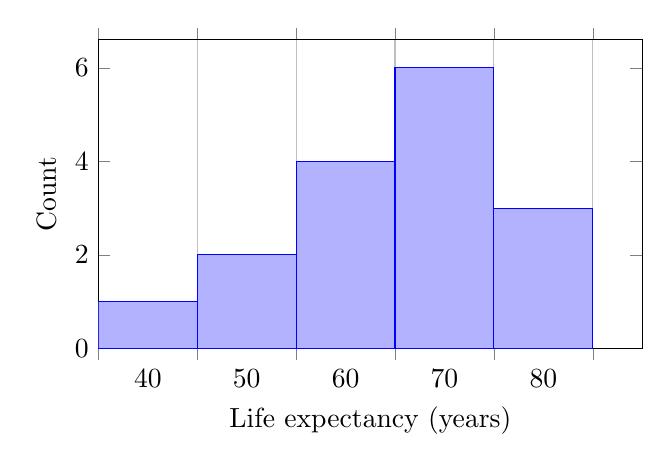
\begin{tikzpicture}
\begin{axis}[width=0.7\textwidth,height=5.5cm,xlabel={Life expectancy (years)},
  ylabel={Count},ybar interval,xmin=40,xmax=95,ymin=0]
\addplot coordinates {(40,1)(50,2)(60,4)(70,6)(80,3)(90,0)};
\end{axis}\end{tikzpicture}
\caption{Illustrative histogram only: replace with your real plot (or embed \texttt{plt.savefig} PNG).}
\end{figure}

\subsection{Bivariate Analysis}
Numeric vs.\ target (scatter + trend), categorical vs.\ target (boxplots by \texttt{status}, \texttt{region}), trend over \texttt{year}.
\figplaceholder{5cm}{Figure: scatter plots of top features vs.\ life expectancy}

\subsection{Correlation Analysis}
Pearson vs.\ Spearman, multicollinearity pairs, chi-square / ANOVA for categorical variables.
\figplaceholder{6cm}{Figure: correlation heatmap}
\begin{table}[H]\centering\caption{Strongest correlations with the target (fill in).}
\begin{tabular}{lrr}\toprule
\textbf{Feature} & \textbf{Pearson} & \textbf{Spearman}\\\midrule
schooling & XX & XX\\ adult\_mortality & XX & XX\\ \dots & & \\\bottomrule
\end{tabular}\end{table}

\subsection{EDA Hypotheses}
\begin{itemize}
\item $H_1$: Higher schooling is associated with higher life expectancy.
\item $H_2$: Developed countries have significantly higher life expectancy.
\item $H_3$: Adult mortality has a strong negative effect.
\end{itemize}

%==================== IV. MODEL DEVELOPMENT ====================
\section{Model Development}
\subsection{Model Selection}
Justify regression and the candidate models (Linear, Ridge/Lasso, Random Forest, Gradient Boosting).

\subsection{Feature Selection}
Drop redundant pairs (e.g.\ \texttt{infant\_deaths} vs.\ \texttt{under\_five\_deaths}); give the rule.

\subsection{Splitting and Scaling}
\begin{lstlisting}
X_tr, X_te, y_tr, y_te = train_test_split(X, y, test_size=0.2, random_state=42)
scaler = StandardScaler().fit(X_tr[num_cols])      # fit on train only
\end{lstlisting}
Note on grouped data: consider splitting by country to avoid leakage across years.

\subsection{Baseline and Training}
Mean-prediction baseline RMSE, then each model's settings.

\subsection{Hyperparameter Tuning}
\begin{lstlisting}
GridSearchCV(Ridge(), {"alpha":[0.01,0.1,1,10,100]}, cv=5,
             scoring="neg_root_mean_squared_error")
\end{lstlisting}

%==================== V. RESULTS ====================
\section{Results and Evaluation}
\subsection{Model Comparison}
\begin{table}[H]\centering\caption{Test-set performance (fill in).}
\begin{tabular}{lcccc}\toprule
\textbf{Model} & \textbf{Train RMSE} & \textbf{CV RMSE} & \textbf{Test RMSE} & \textbf{Test $R^2$}\\\midrule
Baseline (mean) & XX & -- & XX & 0.00\\
Linear Regression & XX & XX & XX & XX\\
Ridge (tuned) & XX & XX & XX & XX\\
Random Forest & XX & XX & XX & XX\\
Gradient Boosting & XX & XX & XX & XX\\\bottomrule
\end{tabular}\end{table}
Interpret: overfitting (train vs.\ test gap), best model and why.

\subsection{Predicted vs.\ Actual and Residuals}
\figplaceholder{5cm}{Figure: predicted vs.\ actual scatter and residual plot}

\subsection{Feature Importance / Coefficients}
\figplaceholder{5cm}{Figure: top coefficients or permutation importance}
Link back to the EDA hypotheses $H_1$--$H_3$: supported or not.

%==================== VI. CONCLUSION ====================
\section{Conclusion and Business Implications}
\subsection{Key Findings}
\begin{enumerate}
\item Finding 1 with a number.
\item Finding 2 with a number.
\end{enumerate}
\subsection{Implications}
Who can use this (health ministries, NGOs, development agencies) and how.
\subsection{Limitations}
Imputed values, country-level aggregates (ecological fallacy), correlation $\neq$ causation, years pooled.
\subsection{Future Work}
Panel/time-series models, more recent data, interaction terms.

%==================== REFERENCES / APPENDIX ====================
\section{References}
\begin{enumerate}
  \item Kumar Rajarshi. (n.d.). \emph{Life Expectancy (WHO)} [Data set]. Kaggle.
        \url{https://www.kaggle.com/datasets/kumarajarshi/life-expectancy-who}.
        Accessed: ...
  \item World Health Organization. \emph{Global Health Observatory data repository}
        (original source of the health indicators).
        \url{https://www.who.int/data/gho}. Accessed: ...
  \item Hoerl, A.\ E., \& Kennard, R.\ W. (1970). Ridge regression: Biased estimation
        for nonorthogonal problems. \emph{Technometrics}, 12(1), 55--67.
  \item Breiman, L. (2001). Random forests. \emph{Machine Learning}, 45, 5--32.
  \item Friedman, J.\ H. (2001). Greedy function approximation: A gradient boosting
        machine. \emph{The Annals of Statistics}, 29(5), 1189--1232.
  \item McKinney, W. (2010). Data structures for statistical computing in Python.
        In \emph{Proceedings of the 9th Python in Science Conference} (pp.\ 56--61).
  \item Harris, C.\ R., Millman, K.\ J., van der Walt, S.\ J., et al.\ (2020).
        Array programming with NumPy. \emph{Nature}, 585, 357--362.
  \item Hunter, J.\ D. (2007). Matplotlib: A 2D graphics environment.
        \emph{Computing in Science \& Engineering}, 9(3), 90--95.
  \item Waskom, M.\ L. (2021). seaborn: Statistical data visualization.
        \emph{Journal of Open Source Software}, 6(60), 3021.
  \item Virtanen, P., Gommers, R., Oliphant, T.\ E., et al.\ (2020). SciPy 1.0:
        Fundamental algorithms for scientific computing in Python.
        \emph{Nature Methods}, 17, 261--272.
  \item Pedregosa, F., Varoquaux, G., Gramfort, A., et al.\ (2011). Scikit-learn:
        Machine learning in Python. \emph{Journal of Machine Learning Research},
        12, 2825--2830.
\end{enumerate}

\section{Appendix}
\begin{enumerate}
  \item Source code link: \url{https://github.com/...}
  \item Dataset link: \url{https://www.kaggle.com/datasets/kumarajarshi/life-expectancy-who}
  \item Data dictionary (variable names after cleaning):
  \begin{itemize}
    \item \texttt{country} (qualitative): country name
    \item \texttt{year} (ordinal): year of observation, 2000--2015
    \item \texttt{status} (qualitative): Developed or Developing
    \item \texttt{life\_expectancy} (quantitative, \textbf{target}): life expectancy at birth, in years
    \item \texttt{adult\_mortality} (quantitative): adult mortality rate, both sexes, per 1000 population
    \item \texttt{infant\_deaths} (quantitative): number of infant deaths per 1000 population
    \item \texttt{alcohol} (quantitative): alcohol consumption per capita, in litres of pure alcohol
    \item \texttt{percentage\_expenditure} (quantitative): health expenditure as \% of GDP per capita
    \item \texttt{hepatitis\_b} (quantitative): Hepatitis B immunization coverage, \%
    \item \texttt{measles} (quantitative): reported measles cases per 1000 population
    \item \texttt{bmi} (quantitative): average body mass index of the population
    \item \texttt{under\_five\_deaths} (quantitative): deaths under age five per 1000 population
    \item \texttt{polio} (quantitative): polio immunization coverage, \%
    \item \texttt{total\_expenditure} (quantitative): government health expenditure as \% of total government expenditure
    \item \texttt{diphtheria} (quantitative): diphtheria (DTP3) immunization coverage, \%
    \item \texttt{hiv\_aids} (quantitative): deaths per 1000 live births due to HIV/AIDS, ages 0--4
    \item \texttt{gdp} (quantitative): gross domestic product per capita, in USD
    \item \texttt{population} (quantitative): population of the country
    \item \texttt{thinness\_1\_19\_years} (quantitative): prevalence of thinness among ages 10--19, \%
    \item \texttt{thinness\_5\_9\_years} (quantitative): prevalence of thinness among ages 5--9, \%
    \item \texttt{income\_composition} (quantitative): income composition of resources, index from 0 to 1
    \item \texttt{schooling} (quantitative): average years of schooling
    % --- engineered columns: edit or delete ---
    \item \texttt{region} (qualitative, engineered): region derived from country
    \item \texttt{period} (qualitative, engineered): year grouped into periods
    \item \texttt{income\_tier} (qualitative, engineered): GDP group (low/medium/high)
  \end{itemize}
  \item Sample of the raw data: insert a screenshot of \texttt{data.head(10)}.
  \item Supplementary figures and tables: extra plots, the full missing-value table, the full coefficient table, tuning results.
\end{enumerate}
\end{document}
